%%%%%%%%%%%%%%%%%%%%%%%%%%%%%%%%%%%%%%%%%%%%%%%%%%%%%%%%%%%%%%%%%%%%%%%%

%%% LaTeX Template for ECAI Papers
%%% Prepared by Ulle Endriss (version 1.0 of 2023-12-10)

%%% To be used with the ECAI class file ecai.cls.
%%% You also will need a bibliography file (such as mybibfile.bib).

%%%%%%%%%%%%%%%%%%%%%%%%%%%%%%%%%%%%%%%%%%%%%%%%%%%%%%%%%%%%%%%%%%%%%%%%

%%% Start your document with the \documentclass{} command.
%%% Use the first variant for the camera-ready paper.
%%% Use the second variant for submission (for double-blind reviewing).

\documentclass{ecai}
%\documentclass[doubleblind]{ecai}

%%%%%%%%%%%%%%%%%%%%%%%%%%%%%%%%%%%%%%%%%%%%%%%%%%%%%%%%%%%%%%%%%%%%%%%%

%%% Load any packages you require here.

\usepackage{latexsym}
\usepackage{amssymb}
\usepackage{amsmath}
\usepackage{amsthm}
\usepackage{booktabs}
\usepackage{enumitem}
\usepackage{graphicx}
\usepackage{color}
\usepackage{tikz} % Added TikZ package for diagrams
\usepackage{algorithm} % Added for algorithm environment
\usepackage{algpseudocode} % Added for algorithmic environment
\usepackage{url} % Added for URL formatting

%%%%%%%%%%%%%%%%%%%%%%%%%%%%%%%%%%%%%%%%%%%%%%%%%%%%%%%%%%%%%%%%%%%%%%%%

%%% Define any theorem-like environments you require here.

\newtheorem{theorem}{Theorem}
\newtheorem{lemma}[theorem]{Lemma}
\newtheorem{corollary}[theorem]{Corollary}
\newtheorem{proposition}[theorem]{Proposition}
\newtheorem{fact}[theorem]{Fact}
\newtheorem{definition}{Definition}

%%%%%%%%%%%%%%%%%%%%%%%%%%%%%%%%%%%%%%%%%%%%%%%%%%%%%%%%%%%%%%%%%%%%%%%%

%%% Define any new commands you require here.

\newcommand{\BibTeX}{B\kern-.05em{\sc i\kern-.025em b}\kern-.08em\TeX}

%%%%%%%%%%%%%%%%%%%%%%%%%%%%%%%%%%%%%%%%%%%%%%%%%%%%%%%%%%%%%%%%%%%%%%%%

\begin{document}

%%%%%%%%%%%%%%%%%%%%%%%%%%%%%%%%%%%%%%%%%%%%%%%%%%%%%%%%%%%%%%%%%%%%%%%%

\begin{frontmatter}

%%% Use this command to specify your submission number.
%%% In doubleblind mode, it will be printed on the first page.

\paperid{123}

%%% Use this command to specify the title of your paper.

\title{Masala Mamu : Agentic AI Kitchen Assistant}

%%% Use this combinations of commands to specify all authors of your
%%% paper. Use \fnms{} and \snm{} to indicate everyone's first names
%%% and surname. This will help the publisher with indexing the
%%% proceedings. Please use a reasonable approximation in case your
%%% name does not neatly split into "first names" and "surname".
%%% Specifying your ORCID digital identifier is optional.
%%% Use the \thanks{} command to indicate one or more corresponding
%%% authors and their email address(es). If so desired, you can specify
%%% author contributions using the \footnote{} command.
\author[A,B]{\fnms{Barani}~\snm{Ranjan S}}
\author[A,B]{\fnms{Brijgopal}~\snm{Bharadwaj}}
\author[A,B]{\fnms{M Chandan Kumar}~\snm{Rao}}
\author[A,B]{\fnms{Shunmuga}~\snm{Janani A}}
\author[A,B]{\fnms{Siva}~\snm{S}}
\address[A]{Division of Interdisciplinary Sciences}
\address[B]{Indian Institute of Science, Bangalore}
%%% Use this environment to include an abstract of your paper.

\begin{abstract}
Modern households struggle with kitchen management tasks like grocery tracking, meal planning, and dietary monitoring. We present Masala Mamu, an AI-powered kitchen assistant using a multi-agent system to integrate these functions. A central Router Agent delegates tasks to specialized agents: Inventory Manager (tracks ingredients), Price Comparison Agent (finds deals across vendors), Recipe Generator (suggests meals based on inventory), and Health \& Diet Agent (monitors nutrition). Built on LangChain/LangGraph with multimodal capabilities, the system offers an integrated approach to meal planning and grocery shopping optimized for Indian dietary preferences and e-commerce landscape.

\smallskip
\noindent\small{\textbf{Project Code:} \url{https://github.com/chandanraoiisc/masala-mamu-agent-ai}}
\end{abstract}

\end{frontmatter}

\section{Introduction}

Maintaining a balanced diet while managing costs presents significant challenges. Existing solutions separately address nutrition tracking, recipe generation, or price comparison, creating fragmented experiences. Masala Mamu integrates these functions for the Indian context, where diverse dietary preferences and a complex e-commerce landscape complicate decision-making.

Key contributions include:
\begin{itemize}[noitemsep,topsep=0pt]
    \item A multi-agent routing architecture for specialized task delegation
    \item A recipe generation system that considers inventory and dietary preferences
    \item A nutrition analysis system with macro-nutrient breakdown capabilities
    \item A price comparison agent for major Indian e-commerce platforms
    \item Vision-based inventory management with semantic search
    \item Real-time nutrition tracking dashboard with personalized insights
\end{itemize}

\section{System Architecture}

\subsection{Multi-Agent Architecture}

Masala Mamu uses specialized agents coordinated by a central router:

\begin{figure}[h]
\centering
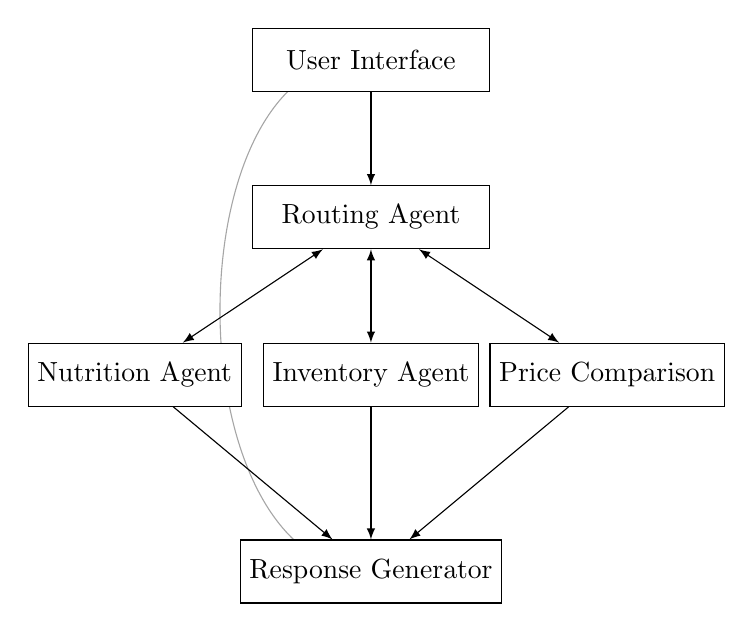
\begin{tikzpicture}[>=latex] % Use latex arrow style which is very clear

    % Draw the curved arrow first (will be behind everything)
    \draw[->, gray!70, thin] (0,-6.5) to[out=180,in=180] (0,0);

    % Define the nodes with opaque backgrounds and borders
    \node[rectangle, draw, fill=white, minimum width=3cm, minimum height=0.8cm] (user) at (0,0) {User Interface};
    \node[rectangle, draw, fill=white, minimum width=3cm, minimum height=0.8cm] (router) at (0,-2) {Routing Agent};
    \node[rectangle, draw, fill=white, minimum width=2cm, minimum height=0.8cm] (nutrition) at (-3,-4) {Nutrition Agent};
    \node[rectangle, draw, fill=white, minimum width=2cm, minimum height=0.8cm] (inventory) at (0,-4) {Inventory Agent};
    \node[rectangle, draw, fill=white, minimum width=2cm, minimum height=0.8cm] (price) at (3,-4) {Price Comparison};
    \node[rectangle, draw, fill=white, minimum width=2cm, minimum height=0.8cm] (response) at (0,-6.5) {Response Generator};

    % Draw all other arrows on top with bold style
    \draw[->] (user) -- (router);
    \draw[<->] (router) -- (nutrition);
    \draw[<->] (router) -- (inventory);
    \draw[<->] (router) -- (price);
    \draw[->] (nutrition) -- (response);
    \draw[->] (inventory) -- (response);
    \draw[->] (price) -- (response);
\end{tikzpicture}
\caption{Multi-agent system architecture}
\end{figure}

\begin{itemize}[noitemsep,topsep=0pt]
    \item \textbf{Routing Agent:} Directs workflows based on query intent and task state
    \item \textbf{Recipe Agent:} Generates meal suggestions based on inventory, dietary, and cuisine preferences
    \item \textbf{Nutrition Agent:} Processes food queries and provides nutritional data
    \item \textbf{Price Agent:} Finds best grocery deals across e-commerce platforms
    \item \textbf{Inventory Agent:} Manages kitchen ingredients database
    \item \textbf{Response Generator:} Creates cohesive responses from agent outputs
\end{itemize}

LangGraph orchestration enables complex multi-domain queries like "What's the most cost-effective high-protein vegetarian meal?"

\subsection{Technology Stack}

\begin{itemize}[noitemsep,topsep=0pt]
    \item \textbf{LLMs:} OpenAI, Gemini, GitHub Marketplace Models
    \item \textbf{Framework:} LangChain/LangGraph for orchestration
    \item \textbf{Frontend:} Streamlit for UI and visualizations
    \item \textbf{Storage:} SQLite (nutrition), MongoDB (inventory)
    \item \textbf{Vision:} GPT-4o for ingredient recognition
    \item \textbf{Embeddings:} Sentence-transformers for semantic search
    \item \textbf{Scraping:} Custom tools for e-commerce price comparison
\end{itemize}

\section{Key Components}

\subsection{Routing Engine}

The LangGraph router flow powers the system's execution logic. An IntentParser using GPT extracts query intents, key entities, and determines agent sequencing. The router, the entry point for queries, tracks required and completed agents to select the next one to activate.

Each agent functions as a node in the graph, processing its specialized task before updating the state and returning control to the router. This creates a conditional execution flow based on user intent that invokes the response generator when complete. This modular approach ensures goal-driven execution and easy extensibility.

\subsection{Nutrition Analysis System}

The nutrition analysis component provides macro-nutrient information through an LLM-powered approach with search augmentation for up-to-date data:

\begin{algorithm}
\caption{Nutrition Analysis Workflow}
\begin{algorithmic}[1]
\State Parse query (recipe vs. ingredients)
\State Initialize LLM with nutrition prompt
\State Perform web search for nutrition data
\State Extract structured data with Pydantic
\State Store in SQLite database with timestamp
\State Generate visualizations of trends
\end{algorithmic}
\end{algorithm}

Key technical features include:

\begin{itemize}[noitemsep,topsep=0pt]
    \item \textbf{Search Augmentation:} Custom DuckDuckGo wrapper for nutrition data retrieval

    \item \textbf{Source Tracking:} Attribution system for data provenance and transparency

    \item \textbf{Cooking Method Awareness:} Adjusts nutrition based on cooking techniques

    \item \textbf{Structured Data Models:} Pydantic models (MacroNutrient, IngredientNutrition)

    \item \textbf{Indian Cuisine Support:} Regional ingredient recognition and unit conversion
\end{itemize}

The relational SQLite database enables historical analysis with per-ingredient breakdowns, supporting comprehensive analytics through the dashboard interface.

\subsection{Price Comparison Engine}

The price comparison engine scrapes real-time pricing from Indian e-commerce platforms (BigBasket, BlinkIt, Zepto, JioMart) using custom tools and suggests alternatives based on price and nutritional similarity. Data is presented comparatively for informed purchasing decisions.

\subsection{Kitchen Inventory Management}

The inventory management module tracks groceries and quantities using:
\begin{itemize}[noitemsep,topsep=0pt]
    \item GPT-4o vision for identifying groceries from images and bill receipt
    \item Vector embeddings for semantic search capabilities
\end{itemize}

In MongoDB, Inventory collection has ItemNm and it’s corresponding quantity with its stored on date as fields. Along with this, an embedding field is also added with the embedded ItemNm in 384 dim vector space. A vector search index is generated on this embedding field in MongoDB. The vector search index is used as the vector store in RAG pipeline.

Users can upload grocery photos or receipts for automatic item detection, with review options before database addition. The RAG-based query system enables natural language inventory questions like "What ingredients do I have for pasta?" or "Which vegetables will expire soon?"

\subsection{Recipe Generation Service}

The recipe generation service provides intelligent dish recommendations tailored to available ingredients and user preferences. Key features include:

\begin{itemize}[noitemsep,topsep=0pt]
    \item \textbf{User Preferences Support:} Accounts for dietary restrictions (e.g., vegan, gluten-free) and preferred cuisine types (e.g., Italian, Indian) to generate personalized recipes
    \item \textbf{Structured Response:} Returns recipes in a consistent JSON format, including ingredient quantities and step-by-step instructions
    \item \textbf{Inventory Integration:} Leverages available ingredient data to recommend practical, waste-reducing meal options
    \item \textbf{Missing Ingredient Identification:} Assists the router agent in detecting any missing ingredients and passes this information to the price comparison service, which then recommends the most cost-effective platforms for purchasing them
\end{itemize}

The service uses prompt engineering to ensure contextually relevant, structured recipe outputs. Integration with inventory and shopping services simplifies meal planning while supporting dietary needs and budget-conscious decisions.


\subsection{Nutrition Analytics Dashboard}

The Plotly-powered nutrition dashboard provides detailed nutritional insights through:

\begin{itemize}[noitemsep,topsep=0pt]
    \item \textbf{Macro-nutrient Tracking:}
      \begin{itemize}[noitemsep,topsep=0pt]
        \item Multi-panel time-series of calories, protein, carbs, and fat
        \item Configurable date ranges (7-90 days) with target value indicators
      \end{itemize}

    \item \textbf{Nutritional Balance:}
      \begin{itemize}[noitemsep,topsep=0pt]
        \item Macro-nutrient distribution pie charts with ratio analysis
        \item Caloric source breakdown with percentage calculations
      \end{itemize}

    \item \textbf{Interactive Features:}
      \begin{itemize}[noitemsep,topsep=0pt]
        \item Customizable nutritional targets and data filtering
        \item Export options for reports and multi-user support
        \item Consistency tracking to identify gaps in nutrition records
      \end{itemize}
\end{itemize}

Built with Streamlit and connected directly to the SQLite database, the dashboard dynamically updates charts based on the latest nutrition data, providing immediate visual feedback on dietary patterns and trends.

\section{Implementation Details}

\subsection{Nutrition Agent Implementation}

The nutrition agent uses LangChain's framework with:

\begin{itemize}[noitemsep,topsep=0pt]
    \item \textbf{System Prompt:} Specialized prompt with structured output requirements and explicit guidance on nutrition analysis

    \item \textbf{Function-Calling Architecture:} OpenAI functions with custom NutritionSearchTool for ingredient and recipe queries

    \item \textbf{Data Models:} Pydantic models (MacroNutrient, IngredientNutrition, RecipeNutrition) for structured data handling

    \item \textbf{Processing Pipeline:} Query classification, web search, data consolidation, and unit normalization
\end{itemize}

Router integration is handled through a NutritionAgentRouter class that manages intent detection, conversation context, and structured responses compatible with the response generator.

Data extraction features include:

\begin{itemize}[noitemsep,topsep=0pt]
    \item Optimized search queries for nutrition databases
    \item LLM-based extraction from semi-structured content
    \item Unit conversion for international and Indian measurements
    \item Error handling with fallback mechanisms
\end{itemize}

The implementation stores both raw and processed data for auditability while providing accurate nutrition information with source citations.

\subsection{Database Schema}

The Nutrition-Agent SQLite database includes three key tables:
\begin{itemize}[noitemsep,topsep=0pt]
    \item \textbf{nutrition\_inquiries:} Query metadata with timestamps and user identifiers
    \item \textbf{nutrition\_records:} Recipe/ingredient macro-nutrient data with foreign keys to inquiries
    \item \textbf{ingredient\_records:} Detailed per-ingredient nutrition with standardized units
\end{itemize}

This relational design enables time-series analysis of nutrition patterns, per-ingredient nutritional impact assessment, data integrity through foreign key constraints, and optimized queries for dashboard visualizations. Database utility functions abstract complex queries while maintaining performance with large datasets spanning months of nutrition records.

\subsection{Routing Logic}

The routing logic is implemented using LangGraph, starting at a router node that evaluates the state and determines the next agent to activate.
\begin{enumerate}[noitemsep,topsep=0pt]
    \item \textbf{Router Initialization:} Defined as a conditional edge that routes based on required\_agents and completed\_agents.
    \item \textbf{Agent Registration:} Agents are added as nodes with async handlers to process input and return updated state.
    \item \textbf{Looping Execution:} After each agent runs, control returns to the router to evaluate the next step.
    \item \textbf{State Management:} Agents append themselves to completed\_agents and add structured outputs (e.g., recipe\_data, inventory\_data).
    \item \textbf{Extensibility:} New agents can be added without modifying router logic—only update the IntentParser.
\end{enumerate}

\subsection{Response Generator}

The ResponseGeneratorAgent reads the current state and parsed intent to understand the user's query and the agents involved in processing it. Based on this, it selectively parses outputs such as recipe\_data, inventory\_data, shopping\_data, and health\_data, depending on which agents were used.

It constructs a structured response tailored to the user's request by including only the relevant sections—e.g., a recipe if the user asked for one, or nutritional data if health advice was sought. This ensures precision and relevance in the system's responses while maintaining a cohesive user experience across multiple agent interactions.

\section{Evaluation}

The system was evaluated on several dimensions:

\subsection{OCR and Image Recognition Accuracy}

Used OCR Readers for reading the grocery bills and handwritten texts, easyOCR as a standalone detected meaningless vegetable names by combining texts, easyOCR with an embedding pipeline to extract just vegetables and fruits, worked better, but still had issues with image noise and handwritten texts. Gpt-4O performed much better with very low WER and CER as shown in Table \ref{tab:ocr_metrics}. A dataset of synthetic bills with handwritten text format and noisy images are generated and used for this comparison.

\begin{table}[ht]
\centering
\resizebox{\columnwidth}{!}{%
\begin{tabular}{|l|c|c|c|c|c|c|}
\hline
\textbf{Model} & \textbf{WER (D1)} & \textbf{CER (D1)} & \textbf{WER (D2)} & \textbf{CER (D2)} & \textbf{WER (D3)} & \textbf{CER (D3)} \\
\hline
GPT-4o & \textbf{0.1182} & \textbf{0.0745} & \textbf{0.1044} & \textbf{0.0583} & \textbf{0.0880} & \textbf{0.0577} \\
EasyOCR + Embedding Pipeline & 0.5508 & 0.3751 & 0.5580 & 0.3839 & 0.5586 & 0.3819 \\
\hline
\end{tabular}%
}
\caption{Comparison of OCR accuracy using Word Error Rate (WER) and Character Error Rate (CER) metrics}
\label{tab:ocr_metrics}
\end{table}

Similarly, a dataset of different vegetables is crawled from web for comparing different models for image detection. A clip model using a small patch and large patch of openAI Vit pretrained model is compared with gpt-4O.
Clip model with large patch performed much better with higher accuracy but failed in distinguishing alike items eg: Peas vs Beans. Gpt-4o performed with full accuracy in identifying individual as well as group of vegetables which are declutterred. Table \ref{tab:ocr_image_accuracy} shows the comparison of accuracy metrics for different models on these datasets.

\begin{table}[ht]
\centering
\begin{tabular}{|l|c|c|c|}
\hline
\textbf{Model} & \textbf{Dataset 1} & \textbf{Dataset 2} & \textbf{Dataset 3} \\
\hline
CLIP (ViT-B/32, small patch) & 0.72 & 0.82 & 0.81 \\
CLIP (ViT-L/14, large patch) & 0.92 & 0.93 & 0.94 \\
GPT-4o (Vision + Multimodal) & \textbf{0.97} & \textbf{0.97} & \textbf{0.98} \\
\hline
\end{tabular}
\caption{Comparison of image recognition accuracy across different models and datasets}
\label{tab:ocr_image_accuracy}
\end{table}

\subsection{Recipe Generation Accuracy}

Recipe generation capabilities were evaluated across four large language models on three datasets of varying complexity and cuisine types. As shown in Table \ref{tab:recipe_accuracy}, smaller, well-optimized models outperformed larger ones in this specialized domain.

\begin{table}[ht]
\centering
\resizebox{\columnwidth}{!}{%
\begin{tabular}{|l|c|c|c|}
\hline
\textbf{Model} & \textbf{Dataset 1} & \textbf{Dataset 2} & \textbf{Dataset 3} \\
\hline
xai/grok-3-mini & \textbf{0.99} & 0.95 & \textbf{0.96} \\
mistral-ai/Ministral-3B & 0.97 & 0.93 & 0.94 \\
meta/Meta-Llama-3.1-70B-Instruct & 0.68 & 0.64 & 0.70 \\
microsoft/Phi-3.5-MoE-instruct & \textbf{0.99} & \textbf{0.97} & \textbf{0.96} \\
\hline
\end{tabular}%
}
\caption{Comparison of recipe generation accuracy across different LLMs and datasets}
\label{tab:recipe_accuracy}
\end{table}

Both xai/grok-3-mini and microsoft/Phi-3.5-MoE-instruct demonstrated exceptional accuracy (above 0.95) across all datasets. The mistral-ai/Ministral-3B model also performed well with slightly lower but reliable scores. Surprisingly, the significantly larger meta/Meta-Llama-3.1-70B-Instruct model showed substantially lower accuracy (0.64–0.70), indicating that architecture specialization and training optimization are more important than model size for domain-specific tasks like recipe generation.

\section{Conclusion \& Future Work}

Masala Mamu demonstrates the effectiveness of multi-agent kitchen assistance, combining nutrition awareness with price optimization in a unified interface. The modular architecture enables future expansion.

Future work:
\begin{itemize}[noitemsep,topsep=0pt]
    \item Enhanced image recognition for receipts/food photos
    \item Nutrition-goal-based recipe recommendations
    \item Long-term dietary pattern analysis
    \item Meal planning and grocery delivery integration
\end{itemize}

\bibliographystyle{ieeetr}
\begin{thebibliography}{9}
\bibitem{langchain} LangChain Framework Documentation, 2023.
\bibitem{langgraph} LangGraph: Graph-based Multi-agent Orchestration, 2024.
\bibitem{streamlit} Streamlit: The fastest way to build data apps, 2022.
\bibitem{confident} Confident AI, "LLM Evaluation Metrics", \url{https://documentation.confident-ai.com/llm-evaluation/metrics/create-locally}, 2023.
\bibitem{github-models} GitHub Marketplace Models, \url{https://github.com/marketplace/models}, 2024.
\end{thebibliography}

\clearpage
\section*{Individual Contributions}

\subsection*{Barani Ranjan S}
\textit{Master of Technology (Online) - DSBA}

[Individual contribution paragraph to be added]

\subsection*{Brijgopal Bharadwaj}
\textit{Master of Technology (Online) - DSBA}

Led the development of the nutrition analysis agent, implementing a comprehensive solution for recipe and ingredient nutrition tracking. Designed and built the multi-LLM compatible agent architecture with search-augmented generation capabilities. Created the database schema for nutrition tracking with SQLite and implemented the Plotly-based visualization dashboard for tracking macro-nutrient consumption over time. Established the router integration layer to enable seamless communication with the broader agent system. Added support for cooking method awareness in nutrition calculations and implemented source citation tracking to ensure transparency and reliability of nutrition data. The resulting system provides accurate, contextualized nutrition analysis with robust historical data capabilities.

\subsection*{M Chandan Kumar Rao}
\textit{Master of Technology (Online) - DSBA}

[Individual contribution paragraph to be added]

\subsection*{Shunmuga Janani A}
\textit{Master of Technology (Online) - DSBA}

[Individual contribution paragraph to be added]

\subsection*{Siva S}
\textit{Master of Technology (Online) - DSBA}

[Individual contribution paragraph to be added]

\clearpage
\section*{Appendix}

\subsection*{Screenshots and Explanations}

\begin{figure}[h]
\centering
\fbox{[Screenshot placeholder: User interface of nutrition dashboard]}
\caption{Nutrition Dashboard: Interactive Plotly-based visualizations for tracking macro-nutrients over time. The dashboard features four primary panels showing calories, protein, carbohydrates, and fat trends with configurable date ranges (7-90 days) and target value indicators. Additional panels show macro-nutrient ratio distributions as pie charts and daily record counts for monitoring tracking consistency. The interface allows users to hover over data points for detailed values and export visualizations for reports.}
\end{figure}

\begin{figure}[h]
\centering
\fbox{[Screenshot placeholder: Price comparison results across e-commerce platforms]}
\caption{Price Comparison Results: The system displays comparative pricing for rice across major Indian e-commerce platforms, highlighting the best deals and providing normalized price-per-unit metrics to enable fair comparison despite different packaging sizes.}
\end{figure}

\begin{figure}[h]
\centering
\fbox{[Screenshot placeholder: Inventory management with image recognition]}
\caption{Inventory Management: The image shows the system correctly identifying various vegetables from an uploaded grocery photo. The interface allows users to review and edit detected items before adding them to their inventory database.}
\end{figure}

\end{document}
